\documentclass[a4paper,11pt]{report}
\usepackage[utf8]{inputenc}
\usepackage[english]{babel}
\usepackage[T1]{fontenc}
\usepackage[gen]{eurosym}
\usepackage{lmodern}

\DeclareUnicodeCharacter{20AC}{\euro{}}

\usepackage[left=1.5cm, right=2cm, top=3cm, bottom=2cm]{geometry}
\setlength{\headsep}{5mm}
\setlength{\headheight}{14pt}
\parindent=0mm
\parskip=3mm

\usepackage{graphicx}
\usepackage{tikz}
\usetikzlibrary{positioning, chains, calc, arrows, decorations.pathreplacing, fit, calc, shapes}
\usepackage{pgfplots}
\usepackage{pgfplotstable}
\pgfplotsset{compat=newest}

% Bachmann–Landau notations
\newcommand{\bigO}[1]{\mathcal O\left( #1 \right)}

% Set symbols
\newcommand{\N}{\mathbb{N}}

% Shortcuts
\newcommand{\set}[1]{\{#1\}}
\newcommand{\zo}{\set{0,1}}
\newcommand{\parens}[1]{\left( #1 \right)}
\newcommand{\intval}[1]{\left\llbracket #1 \right\rrbracket}

\usepackage[acronym,shortcuts,toc,nogroupskip]{glossaries}
\makeglossaries
\usepackage[pdfusetitle,hidelinks]{hyperref}
\usepackage{amsmath,amsthm,amssymb,array,enumerate,cancel,nth,stmaryrd,fancyhdr,titling,mathtools}
\usepackage{units}
\usepackage{enumitem}
\setlist{nolistsep}
\usepackage{tabularx}


\newacronym{fg}{FG}{Factor Graph}
\newacronym{spa}{SPA}{Sum-Product Algorithm}
\newacronym{ldpc}{LDPC}{Low-Density-Parity-Check}
\newacronym{vfm}{VFM}{variable node to factor node message}
\newacronym{fvm}{FVM}{factor node to variable node message}
\newacronym{jit}{JIT}{Just-In-Time}


\newlength\gheight
\newlength\ndist
\newlength\fghskip

\newcommand{\fgargset}[1]{\pgfkeys{/factorgraph/.cd,#1}}
\fgargset{
    height/.store in=\fgheight,
    height=10cm,
    width/.store in=\fgwidth,
    width=5cm,
    variable count/.store in=\fgnbv,
    variable count=1,
    factor count/.store in=\fgnbf,
    factor count=1,
    edges/.store in=\fgedges,
    edges={1/1},
    variable label/.store in=\fgvlabel,
    variable label=$x_{\i}$,
    factor label/.store in=\fgflabel,
    factor label=$f_{\j}$
}

\newcommand{\factorgraph}[1][]{
    \begin{scope}
        \fgargset{#1}
        \pgfmathsetlength\gheight{\fgheight}
        \pgfmathsetlength\fghskip{0}
        \ifnum\fgnbv>1
            \pgfmathsetlength\ndist{\gheight/(\fgnbv-1)}
        \else
            \pgfmathsetlength\ndist{0}
            \ifnum\fgnbf>1
                \pgfmathsetlength\fghskip{-\gheight/2}
            \fi
        \fi
        \begin{scope}[shift={(0,\fghskip)},start chain=1 going {at=(\tikzchainprevious),shift=(-90:\ndist)}]
            \foreach \i in {1,...,\fgnbv} {
                    \node[on chain=1, ellipse, draw] (x_\i) {\fgvlabel};
            }
        \end{scope}
        \pgfmathsetlength\fghskip{0}
        \ifnum\fgnbf>1
            \pgfmathsetlength\ndist{\gheight/(\fgnbf-1)}
        \else
            \ifnum\fgnbv>1
                \pgfmathsetlength\fghskip{-\gheight/2}
            \fi
            \pgfmathsetlength\ndist{0}
        \fi
        \begin{scope}[shift={(\fgwidth,\fghskip)}, start chain=2 going {at=(\tikzchainprevious),shift=(-90:\ndist)}]
            \foreach \j in {1,...,\fgnbf} {
                \node[on chain=2, rectangle, draw] (f_\j) {\fgflabel};
            }
        \end{scope}
        \foreach \i/\j/\k in \fgedges {
            \ifnum\pdfstrcmp{\k}{vfm}=0
                \path (x_\i) -- node[sloped] (m_\i_\j) {$m_{\text{\fgvlabel} \to \text{\fgflabel}}$} (f_\j);
                \draw[-latex] (x_\i) -- (m_\i_\j) -- (f_\j);
            \else
                \ifnum\pdfstrcmp{\k}{fvm}=0
                    \path (x_\i) -- node[sloped] (m_\i_\j) {$m_{\text{\fgflabel} \to \text{\fgvlabel}}$} (f_\j);
                    \draw[-latex] (f_\j) -- (m_\i_\j) -- (x_\i);
                \else
                    \draw[-] (x_\i.east) -- (f_\j.west);
                \fi
            \fi
        }
    \end{scope}
}


\title{Sudoku solving by factor graphs}
\author{Romain Labolle}
\date{2015}

\begin{document}

\pagenumbering{Roman}
\thispagestyle{empty}


\includegraphics[height=2cm]{logos/ens.pdf} \hfill

\includegraphics[height=2cm]{logos/ucbl.pdf} \hfill

\includegraphics[height=2cm]{logos/univlyon.pdf}

\vspace{0.5cm}

\begin{tabularx}{\textwidth}{@{} l X l @{} }
\textsc{Master of Fundamental Computer Science} & & Internship 2014--2015 \\
\textit{École Normale Supérieure de Lyon} & & Romain \textsc{Labolle} \\
\textit{Université Claude Bernard Lyon I} & & Master 1
\end{tabularx}

\begin{center}

\vfill

\rule[11pt]{5cm}{0.5pt}

\textbf{\huge \thetitle}

\rule{5cm}{0.5pt}

\vfill

\vspace{2.5cm}

\parbox{15cm}{
Supervisors :

\textbf{Stephan Pfletschinger} \href{mailto:stephan.pfletschinger@ieee.org}{\tt @ieee.org}

\textbf{Pau Closas} \href{mailto:pau.closas@cttc.cat}{\tt @cttc.cat}

\textbf{Monica Navarro} \href{mailto:monica.navarro@cttc.cat}{\tt @cttc.cat}

Centre Tecnològic de Telecomunicacions de Catalunya (CTTC)

\textit{Parc Mediterrani de la Tecnologia (PMT) - Building B4\\
Av. Carl Friedrich Gauss 7\\
08860 Castelldefels (Spain)}

\url{http://www.cttc.cat/}
}

\vspace{1.5cm}

\hfill
%
\includegraphics[height=3cm]{logos/cttc.png}
%\hfill

\includegraphics[height=3cm]{logos/cttc.png}
%\hfill
%
\includegraphics[height=3cm]{logos/cttc.png}
\hfill \null

\end{center}


\tableofcontents
\newpage

\pagenumbering{arabic}

\pagestyle{fancy}
\fancyhead[L]{\thetitle} 
\fancyhead[R]{\nouppercase{\textsl{\leftmark}}}

\chapter{Introduction}

The goal of this internship was to study the \acl{spa} on \aclp{fg}, an algorithm that can be used to express and solve many different kinds of problems. We especially focused on one example, the Sudoku solving problem, and studied different kinds of optimisations that could be made to the algorithm. Some of the optimisations we found can be them generalized to other problems.

In this document, we first introduce the different notions relative to \aclp{fg} and the \acl{spa}, we then show how it can be applied to the Sudoku solving problem and we finally present different optimisations and the resulting performances.

\chapter{Factor Graphs}

A \ac{fg}\cite{kschischang2001factor} is a bipartite graph that can be used to describe the structure of the factorization of a function. For example, let us consider a function $f(x_1,x_2,x_3,x_4,x_5)$ that can be factorized as: \begin{equation}\label{eq:fgex}
    f(x_1,x_2,x_3,x_4,x_5) = f_1(x_1,x_2) f_2(x_2,x_3) f_3(x_4) f_4(x_4,x_5).
\end{equation}
We can express the structure of this factorization by a \ac{fg}. This is a bipartite graph with variable nodes for each variable $x_{\nu}$ on one side and factor nodes for each local function $f_{\mu}$ on the other side, with an edge between $x_{\nu}$ and $f_{\mu}$ if and only if $f_{\mu}$ is a function of $x_{\nu}$.

The \ac{fg} corresponding to the example \eqref{eq:fgex} is shown in figure \ref{fig:fgex}. The typical representation uses squares for factor nodes and circles for variable nodes.

\begin{figure}[!ht]
    \centering
    \begin{tikzpicture}[baseline=(current bounding box.north)]
        \factorgraph[
            variable count=5,
            factor count=4,
            height=5cm,
            width=5cm,
            edges={1/1,2/1,2/2,3/2,4/3,4/4,5/4}
        ]
    \end{tikzpicture}
    \caption{Example \acl{fg} corresponding to the function in \eqref{eq:fgex}}
    \label{fig:fgex}
\end{figure}

This type of problem representation is very useful in, for instance, large systems over which it might be difficult to make inference. Using \ac{fg} theory and tools, we can divide a complex problem into small pieces that are easier to deal with by accounting for the variables' dependencies.

Furthermore, it allows for an iterative solution that reduces complex problems into feasible implementations.

\section{Sum-Product Algorithm}

In \acp{fg}, one is typically interested in making inferences about the marginal function of each variable node. This could be complex in general, but \ac{fg} theory provide a powerful framework.

The \ac{spa}\cite{kschischang2001factor} is a message-passing algorithm working on \acp{fg}. It is a generalization of algorithms used in many domains such as \ac{ldpc} decoding, Belief Propagation on Bayesian networks, Kalman filtering, etc. There is no assumption about messages passed between the nodes and it can be, for example, sets of possible values, probability mass functions or probability density functions. In the following sections, we will mainly use messages representing probability distribution: sets of possible values or probability vector in discrete cases, parameters of a Gaussian distribution, …

\subsection{Message-passing rules}
In order to compute the messages passed from one node to another we follow different rules described in \cite{kschischang2001factor}. A given message from a node $a$ to a node $b$ depends on messages received by $a$ from all its neighbors except $b$. An example is shown in figure \ref{fig:spampex}.

\begin{figure}[!ht]
    \centering
    \begin{tikzpicture}[baseline=(current bounding box.north)]
        \factorgraph[
            variable count=4,
            factor count=1,
            height=5cm,
            width=7cm,
            edges={1/1/vfm,2/1/vfm,3/1/vfm,4/1/fvm}
        ]
        \node[right=of f_1,text width=4cm,cloud, cloud puffs=15, cloud ignores aspect, align=center, draw] {Compute $m_{f_1 \to x_4}$ from the values of $m_{x_1\to f_1}$, $m_{x_2\to f_1}$ and $m_{x_3\to f_1}$};
    \end{tikzpicture}
    \caption{\ac{spa}: example message-passing on a \ac{fg}, message generated from factor node $f_1$ to variable node $x_4$}
    \label{fig:spampex}
\end{figure}


\subsubsection{Variable node to factor node messages}

\Acp{vfm} are the easiest to compute, it's simply the product of all other incoming messages:

\begin{equation}
m_{x \to f} (x) = \prod_{h\in \mathcal{N}(x)\backslash\set{f}} m_{h \to x} (x)
\end{equation}

where $\mathcal{N}(x)$ represent the neighbors of $x$ in the \ac{fg}.


\subsubsection{Factor node to variable node messages}

\Acp{fvm} are more complex to compute:

\begin{equation}
m_{f \to x} (x) = \sum_{\sim\set{x}} f(X) \parens{ \prod_{y\in \mathcal{N}(f)\backslash\set{x}} m_{y \to f} (y) }
\end{equation}

where $X=\mathcal{N}(f)$ represent the neighbors of $f$ in the \ac{fg} and $\sum_{\sim\set{x}}$ is the summary operator described below.

\subsubsection{Termination rule}

The final result of the algorithm for a given variable $x$ is called the marginalization of the function and is given by:

\begin{equation}
m(x) = \prod_{h\in\mathcal{N}(x)} m_{h\to x} (x)
\end{equation}

If the messages being passed are sets of possible values or discrete probability distributions, we can use this marginal function to find an estimate of the corresponding variable, which is the ultimate goal in \acp{fg}.

The termination rule itself depend on the problem. In some cases, we can have a clear termination rule (for example in LDPC decoding, the algorithm terminate when all check nodes are satisfied), in other cases we either have to limit the number of iterations or consider that a message doesn't change anymore once the difference of its value at each iteration have reached a certain threshold.

\subsubsection{The summary operator}

The summary operator $\sum_{\sim\set{x_i}} f(X)$ represent the summary of a function $f$ over all possible values of all variable $x_1,\dots,x_n$ except $x_i$. Depending on the definition domain of the function $f$, it can either be a sum $f$ is define over a discrete domain:
\begin{equation}
\sum_{\sim\set{x_i}} f(X) = \sum_{x_1} \dots \sum_{x_{i-1}} \sum_{x_{i+1}} \dots \sum_{x_n} f(x_1,\dots,x_{i-1},x_i,x_{i+1},\dots,x_n)
\end{equation}

or an integral if $f$ is define over a continuous domain:
\begin{equation}
\sum_{\sim\set{x_i}} f(X) = \int\limits_{D_1} \! \dots \! \int\limits_{D_{i-1}} \! \int\limits_{D_{i+1}}\! \dots \! \int\limits_{D_n} \! f(x_1,\dots,x_{i-1},x_i,x_{i+1},\dots,x_n)\, \mathrm{d}x_n \dots \mathrm{d}x_{i+1}\,\mathrm{d}x_{i-1}\dots\mathrm{d}x_1
\end{equation}

where $\sum\limits_{x_k} = \sum\limits_{x_k\in D_k}$, $\int\limits_{D_k} = \int\limits_{x_k\in D_k}$  and $D_k$ is the domain of definition of the function for the $k$-th variable.


\chapter{Sudoku solving}

\section{Presentation of the problem}

Lets consider a $q \times q$ grid subdivided into $q$ sub-grids of size $p \times p$ (with $q=p^2, p\in\N^*$). The goal of the Sudoku game is to fill the grid with numbers from $1$ to $q$ so that each line, each row and each sub-grid contains exactly one of these numbers. In each instance of the game, some cells are already filled in so that there is a unique solution. For regular Sudoku $q=9$, but to simplify the representation, examples will use $q=4$.

We can define the constraint function $\mathcal{C}: \set{1,\dots,q}^{q^2} \to \zo$ for Sudokus that associate to a grid a value of $1$ if it respects all the Sudoku rules and $0$ otherwise. This function can be factorized into a product of $3 \cdot q$ local constraint functions depending only on $q$ variables each:
\begin{equation}\label{eq:sudokuconst}
\mathcal{C}(x_1,\dots,x_{q^2}) = c_1(x_1,\dots,x_q) \cdot c_2(x_{q+1},\dots,x_{2q}) \cdots c_{3q}(\dots)
\end{equation}

The first $q$ functions represent the row constraints, then the column constraint and finally the $q$ last functions represent the sub-grid constraints. Those functions are all the same and return $1$ if and only if all its input arguments are different. In other words, it checks if its input is a permutation of the set $\set{1,\dots,q}$.


\section{Solving Sudokus with the \acl{spa}}

Since the constraint function can be factorized as in \eqref{eq:sudokuconst}, it can be represented as a factor graph (see figure \ref{fig:sudokufg4}).

Then by applying the \ac{spa} over the \ac{fg}, we deduce the marginal functions $m(x_i)$ and find the value of $x_i$ that yields $\mathcal{C}(x_1,\dots,x_{q^2}) = 1$.

In this case, and to simplify the computation, the messages passed across the nodes will be sets of possible values, which can also be seen as probability vectors of size $q$ with all values being either $0$ or $1$ (with a normalization coefficient). Thus the sum of two messages is the union of the sets and the product is the intersection. We initialize the values with the known values of the grid to solve:
\begin{itemize}
\item $x_i = \set{k}$ if the cell $i$ containts $k$
\item $x_i = \set{1,\dots,q}$ if the cell $i$ is empty
\end{itemize}

\begin{figure}[!ht]
    \centering
    \begin{tikzpicture}[baseline=(current bounding box.north)]
        \def\p{2}
        \pgfmathtruncatemacro\q{\p*\p}
        \pgfmathtruncatemacro\nbv{\q*\q}
        \pgfmathtruncatemacro\nbf{3*\q}
        \factorgraph[
            variable count=\nbv,
            factor count=\nbf,
            height=10cm,
            width=8cm,
            edges={},
            factor label=$c_{\j}$
        ]
        \begin{scope}
            \foreach \i in {1,...,\q} {
                \foreach \j in {1,...,\q} {
                    \pgfmathtruncatemacro\cell{\q*(\i-1)+\j}
                    \draw[-] (x_\cell.east) -- (f_\i.west);
                }
            }
            \foreach \i in {1,...,\q} {
                \foreach \j in {1,...,\q} {
                    \pgfmathtruncatemacro\cell{\q*(\i-1)+\j}
                    \pgfmathtruncatemacro\col{\q+\j}
                    \draw[-] (x_\cell.east) -- (f_\col.west);
                }
            }
            \foreach \i in {1,...,\q} {
                \foreach \j in {1,...,\q} {
                    \pgfmathtruncatemacro\cell{\q*(\i-1)+\j}
                    \pgfmathtruncatemacro\sgrid{2*\q+1+int((\i-1)/\p)+int((\j-1)/\p)*\p};
                    \draw[-] (x_\cell.east) -- (f_\sgrid.west);
                }
            }
            \pgfmathtruncatemacro\bstart{1};
            \pgfmathtruncatemacro\bstop{\q};
            \draw[thick,decorate,decoration={brace,amplitude=10pt,raise=10pt}]
                (f_\bstart.north east) -- (f_\bstop.south east)
                node [midway, right,xshift=20pt] {Row constraints};
            \pgfmathtruncatemacro\bstart{\q+1};
            \pgfmathtruncatemacro\bstop{2*\q};
            \draw[thick,decorate,decoration={brace,amplitude=10pt,raise=10pt}]
                (f_\bstart.north east) -- (f_\bstop.south east)
                node [midway, right,xshift=20pt] {Column constraints};
            \pgfmathtruncatemacro\bstart{2*\q+1};
            \pgfmathtruncatemacro\bstop{3*\q};
            \draw[thick,decorate,decoration={brace,amplitude=10pt,raise=10pt}]
                (f_\bstart.north east) -- (f_\bstop.south east)
                node [midway, right,xshift=20pt] {Sub-grid constraints};
            \pgfmathtruncatemacro\bstart{\q*\q};
            \pgfmathtruncatemacro\bstop{1};
            \draw[thick,decorate,decoration={brace,amplitude=10pt,raise=10pt}]
                (x_\bstart.south west) -- (x_\bstop.north west)
                node [midway, left,xshift=-20pt] {Variables};
        \end{scope}
    \end{tikzpicture}
    \caption{\ac{fg} representation of the Sudoku constraint function $\mathcal{C}$ described in \eqref{eq:sudokuconst} for $q=4$ }
    \label{fig:sudokufg4}
\end{figure}



\section{Implementation}

In order to test the algorithm, we have implemented a generic Python class to represent a \ac{fg} and apply the \ac{spa} to it. We have then implemented different optimizations on the way and order in which messages are computed in order to achieve better performance, by simplifying the message computation and by reducing the number of computed messages.

Some of those optimization are specific to the given problem (but very similar optimization might be found for other problems), other are general and might be applied to other instances of the \ac{spa}

\subsection{Original implementation}
\label{sec:orig}

This is the most generic implementation, with almost no assumption on the nature of the \ac{fg}. However, it is relatively slow, mostly due to the time taken by the \acp{fvm} computation. Indeed, in the case of Sudokus, the local function $c_i$ is non zero if its arguments are a valid permutation of $\set{1,\dots,q}$. So in the \ac{fvm} computation, the formula becomes:

\begin{equation}
m_{f \to x} (\mathbf{x}) = \sum_{\sim\set{x}} f(X) \parens{ \prod_{\mathbf{y}\in \mathcal{N}(f)\backslash\set{x}} m_{y \to f} (\mathbf{y}) } = \sum_{X \in \mathfrak{S}_x(\mathbf{x})} \parens{ \prod_{\mathbf{y}\in \mathcal{N}(f)\backslash\set{x}} m_{y \to f} (\mathbf{y}) },
\end{equation}

where $\mathfrak{S}_x(\mathbf{x})$ is the set of all permutations of $\mathcal{N}(f) = \set{1,\dots,q}$ in which the variable $x$ has the value $\mathbf{x}$. Since this involves permutation of all but one variable, we have the $\mathrm{Card}(\mathfrak{S}_x(\mathbf{x})) = (q-1)!$

Therefore, the complexity of the \ac{fvm} computation in this case is $\bigO{q!}$, where $\bigO{\cdot}$ is the big O Landau notation.

We did not implemented the naive algorithm that compute the product even if $f(X) = 0$ since its complexity would have been $\bigO{q^q}$. Indeed, in the naive algorithm, the summary operator iterate over the $q$ possibilities for the $q-1$ variable and thus have to compute $q^{q-1}$ times a product of $q$ messages.


\subsection{Faster message computation}
\label{sec:set}

The \ac{fvm} computation can be simplified by using the following formula \cite{atkins2014density}:

\begin{equation}
m_{f \to x} (\mathbf{x}) = \set{1,\dots,q} - \bigcup\limits_{n} A_n
\end{equation}

Where $A_n$ is any set such that
\begin{equation}
\exists \mathcal{J} \subset \set{1,\dots,q} \text{ such that }
\begin{cases}
x \ne x_j, \forall j \in \mathcal{J}\\
A_n = \bigcup\limits_{j \in \mathcal{J}} m_{x_j \to f} (\mathbf{x_j})\\
\mathrm{Card}(\mathcal{J}) = \mathrm{Card}(A_n)
\end{cases}
\end{equation}

In order to find all the $A_n$, we have to iterate over at most $2^{q-1}$ possible values of $\mathcal{J}$. We hence get a complexity of at most $\bigO{2^q}$.

Moreover if we subtract the $A_n$ as we compute them, we can improve the algorithm a little bit in some cases: if we obtain $m_{f \to x}(\mathbf{x}) = \emptyset$, we can stop searching for other $A_n$ as it will not change the result.

This approach is very close to the technique that is actually used by humans to solve Sudokus: if in a given row (resp. column and sub-grid) there are $k$ cells that can only accept a subset of $k$ values, these values can be removed from the possibilities of all other cells in the row (resp. column and sub-grid). The case $k=1$ removes values already placed in the grid and the case $k=q-1$ complete a line with only 1 remaining cell.

This approach cannot be generalized to all instances of \ac{spa}, but it can actually be used on problems similar to this one where the messages are probabilities that are uniform on their support (and hence can be expressed as sets).

\subsection{Message computation scheduling}
\label{sec:sched}

Messages can actually be computed in any given order and some scheduling might require less message computation in order to converge.

We have seen that \ac{vfm} are fast to compute compared to \ac{fvm}, thus we aim at minimizing the number of \ac{fvm} computations in order to speed up our algorithm.

The scheduling we used for all the previous implementations is the naive one where we first compute all \acp{vfm} and the all \acp{fvm}, as shown in figure \ref{fig:naiveschedule}, and then repeat those two steps until all the messages are stabilized (no message was changed by those two steps).

\begin{figure}[!ht]
    \centering
    \begin{tikzpicture}[baseline=(current bounding box.north)]
        \begin{scope}
            \factorgraph[
                variable count=3,
                factor count=2,
                height=2cm,
                width=4cm,
                edges={1/1/vfm,2/1/vfm,2/2/vfm,3/2/vfm}
            ]
            \node[below=0.5 of m_3_2] {Compute all \acp{vfm} first};
        \end{scope}
    \end{tikzpicture}
    \hspace{1cm}
    \begin{tikzpicture}[baseline=(current bounding box.north)]
        \begin{scope}
            \factorgraph[
                variable count=3,
                factor count=2,
                height=2cm,
                width=4cm,
                edges={1/1/fvm,2/1/fvm,2/2/fvm,3/2/fvm}
            ]
            \node[below=0.5 of m_3_2] {Then all \acp{fvm}};
        \end{scope}
    \end{tikzpicture}
    \caption{Example of naive scheduling on a simple \ac{fg}}
    \label{fig:naiveschedule}
\end{figure}

\subsubsection{Tracking \ac{vfm} changes}
\label{sec:skip}

The first improvement we have implemented is to track \ac{vfm} changes in order to avoid computing twice a \ac{fvm} with the same inputs.

Indeed, especially towards the end of the algorithm when only a small portion of the graph is not stabilized, the naive scheduling was recalculating all the messages at each step even if only a few of them had actually to be computed.

%This improved a lot the performances of our algorithm as shown in the results (Section \ref{sec:results})

\subsubsection{Focusing on \acp{fvm}}

We then changed our scheduler to focus on the \acp{fvm} computation, propagating these messages immediately by computing the affected \acp{vfm} (see figure \ref{fig:fvmfocusedschedule}), in order to take into account the most recent updates for the next \ac{fvm} computation. In this scheduler, the \acp{fvm} are always computed in the same order and we loop through them until the messages stabilize.

The idea here is still to try to reduce the number of \acp{fvm} computations, but this time by taking into account as much information as possible in each computation to make messages converge faster and reducing the number of iterations needed.

We reuse the previous optimization to avoid computing twice the same message. In order to do so, each time a \ac{vfm} change, the destination factor node is marked as outdated for all its neighbors except the one sending the \ac{vfm}, so that we know those \acp{fvm} will have to be recomputed.

%TODO: results

\begin{figure}[!ht]
    \centering
    \begin{tikzpicture}[baseline=(current bounding box.north)]
        \factorgraph[
            variable count=3,
            factor count=2,
            height=2cm,
            width=5cm,
            edges={1/1/fvm,2/1,2/2,3/2}
        ]
    \end{tikzpicture}
    \hspace{1cm}
    \begin{tikzpicture}[baseline=(current bounding box.north)]
        \factorgraph[
            variable count=3,
            factor count=2,
            height=2cm,
            width=5cm,
            edges={1/1,2/1/fvm,2/2/vfm,3/2}
        ]
    \end{tikzpicture}
    
    \vspace{0.5cm}
    
    \begin{tikzpicture}[baseline=(current bounding box.north)]
        \factorgraph[
            variable count=3,
            factor count=2,
            height=2cm,
            width=5cm,
            edges={1/1,2/1/vfm,2/2/fvm,3/2}
        ]
    \end{tikzpicture}
    \hspace{1cm}
    \begin{tikzpicture}[baseline=(current bounding box.north)]
        \factorgraph[
            variable count=3,
            factor count=2,
            height=2cm,
            width=5cm,
            edges={1/1,2/1,2/2,3/2/fvm}
        ]
    \end{tikzpicture}
    \caption{Example of \ac{fvm}-focused scheduling on a simple \ac{fg}}
    \label{fig:fvmfocusedschedule}
\end{figure}


\subsubsection{Reordering the \acp{fvm} computation}

By following this same idea of always integrating the most changes at each \ac{fvm} computation, we implemented 3 different ways of choosing which \ac{fvm} to compute at each step:
\begin{enumerate}
\item \textbf{Number of changed inputs:} we choose to propagate the \ac{fvm} which are marked as outdated by more of its variable nodes. If there are several candidates, we take one of them arbitrarily (the first one by index for example).
\item \textbf{Sum of the changes:} Instead of simply indicating `outdated', the \ac{vfm} computation results in a number representing how much it changed from its previous value. In our case, this number is the number of elements that have been removed from the set of possible values. Then we keep for each \ac{fvm} the sum of all these number of changes and we choose the one with the highest value. We still break ties arbitrarily (e.g., by index).
\item \textbf{A mix of both:} We combine the two previous techniques: we first sort by number of changed inputs, then we break ties with the sum of changes and then arbitrarily (e.g., by index).
\end{enumerate}


\section{Results}
\label{sec:results}

In order to evaluate the efficiency of the different implementations and schedulers, we implemented an operation counter that was able to count the number of additions, multiplications and message computations in each direction. Hence, the resulting statistics doesn't depend on the machine running the tests.
The input data sets was taken from online databases of known hard Sudokus for $9\times 9$\cite{magictour,gordon} and $16 \times 16$\cite{magictour} grids; the $4 \times 4$ grids was extracted from an online Sudoku generator\cite{sugen}.

\subsection{Comparing different implementations}
\label{sec:resimpl}

We compared the original implementation (Section \ref{sec:orig}), the `set-formula' implementation (Section \ref{sec:set}) and the set-formula implementation with message computation skipping (Section \ref{sec:skip}).

The original implementation could only be ran over small $4 \times 4$ Sudoku grids, any larger grid took too much resources to finish properly.

The results for the different grid sizes are shown in figure \ref{fig:resimpl} (whiskers represent minimum and maximum values)

\begin{figure}[!ht]
    \centering
    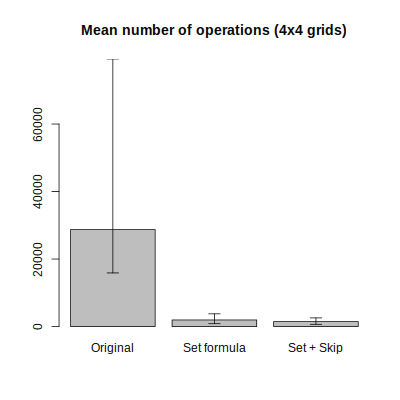
\includegraphics[width=5.8cm]{../Test/results/impl_2_op.png}%
    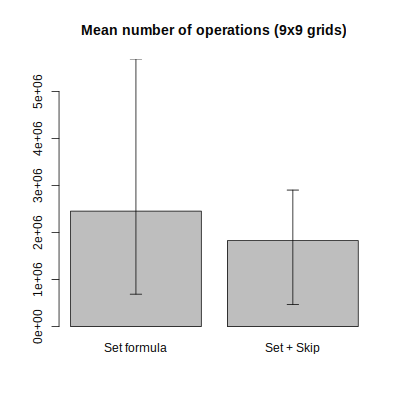
\includegraphics[width=5.8cm]{../Test/results/impl_3_op.png}%
    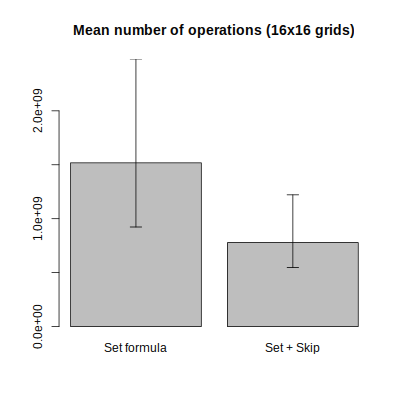
\includegraphics[width=5.8cm]{../Test/results/impl_4_op.png}
    \caption{Comparison of the different implementations}
    \label{fig:resimpl}
\end{figure}

Theses results confirm our expectations.

\subsection{Comparing different schedulers}
\label{sec:ressched}

We now use our best implementation to compare the different message schedulers (Section \ref{sec:sched}). Results are shown in figure \ref{fig:ressched}

\begin{figure}[!ht]
    \centering
    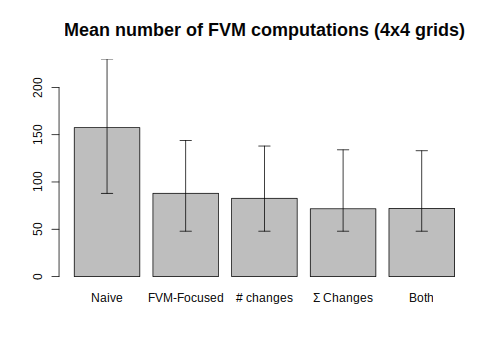
\includegraphics[width=5.8cm]{../Test/results/sched_2_fvm.png}%
    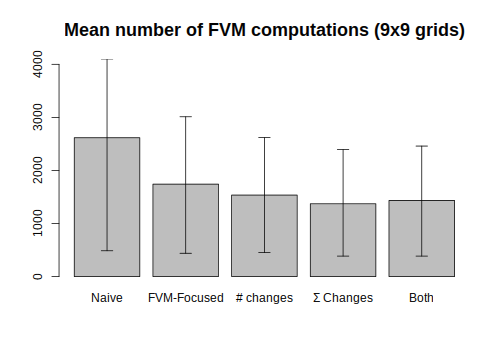
\includegraphics[width=5.8cm]{../Test/results/sched_3_fvm.png}%
    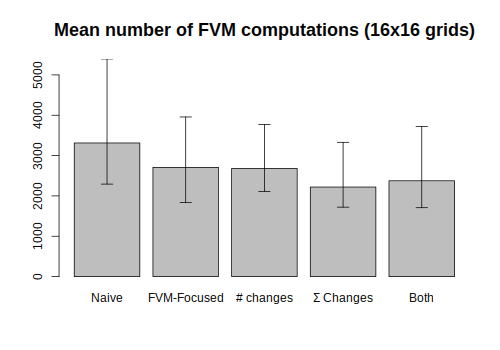
\includegraphics[width=5.8cm]{../Test/results/sched_4_fvm.png}
    
    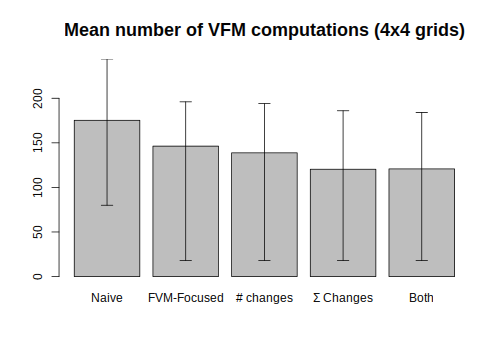
\includegraphics[width=5.8cm]{../Test/results/sched_2_vfm.png}%
    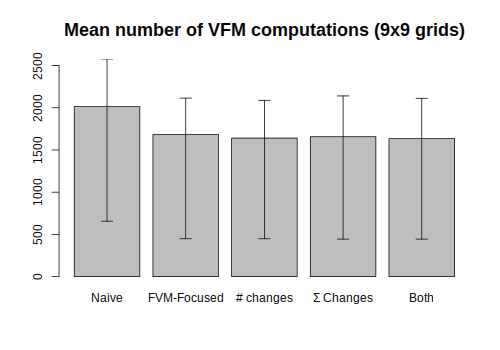
\includegraphics[width=5.8cm]{../Test/results/sched_3_vfm.png}%
    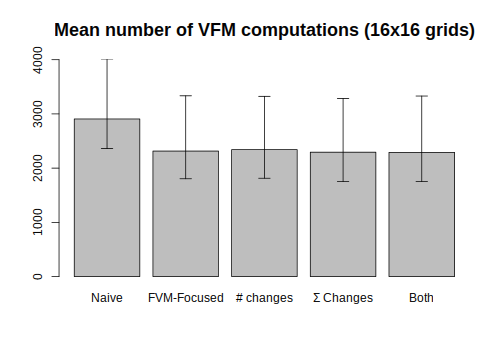
\includegraphics[width=5.8cm]{../Test/results/sched_4_vfm.png}
    
    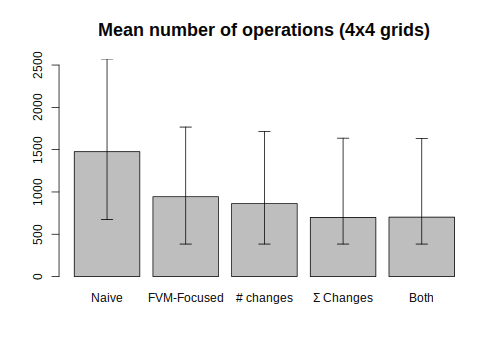
\includegraphics[width=5.8cm]{../Test/results/sched_2_op.png}%
    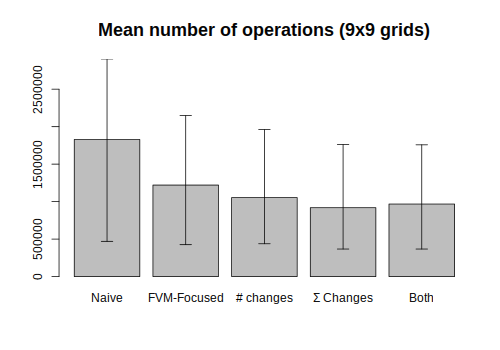
\includegraphics[width=5.8cm]{../Test/results/sched_3_op.png}%
    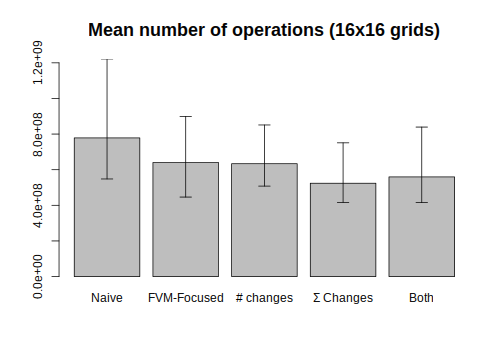
\includegraphics[width=5.8cm]{../Test/results/sched_4_op.png}
    \caption{Comparison of the different schedulers}
    \label{fig:ressched}
\end{figure}

These results show that the FVM-focused approach provides better overall performances (in term of number of operations), but also that it does not even involve more \ac{vfm} computations. Moreover, we can see that the most efficient scheduler is the one based on sum of all changes.

We can see for example that for the 16x16 grids, the "naive" scheduler takes an average of around $780\,000\,000$ operations (additions + multiplications) to complete whereas the "Sum of changes" scheduler only takes about $525\,000\,000$ operations, which represents a reduction of almost $\nicefrac{1}{3}$ of the number of required operations.

\chapter{Conclusions}

The general definition of the \ac{spa} leaves a lot of space to implementation choices, especially regarding the scheduling of the different message computations. And we were indeed able to come up with different implementations leading to different performances.

After analyzing the different results, it came out that we were right in assuming that we could achieve better performances by always computing messages with input that changed the most. Indeed, our best scheduler ("$\Sigma$ changes") is the one that take into account the most information from a message inputs.

This is an interesting result as it is not bound in any way to the problem we were looking at and can be applied to any other \ac{spa} instance.

\section*{Resources}

The source code of the implementation and of this document are available online at \url{http://sudoku.cat/}.

A live demo of the solver can be accessed via the telnet protocol at sudoku.cat on port 23 by running the command \texttt{telnet sudoku.cat}.

\addcontentsline{toc}{chapter}{Bibliography}
\nocite{*}
\bibliographystyle{plain}
\bibliography{biblio}

\end{document}